

Mit diesem Kapitel werden Einblicke in die notwendige Grundlagen zur Realisierung unserer Arbeit gegeben. 
Zuerst werden wir uns mit der Thematik Emotion (Definition und Klassifikation) beschäftigen. 
Im Weiteren werden ``Virtual Reality'' ( beziehungsweise HTC Vive VR-Brille) genauer erklärt. 
Ebenfalls kommt eine Erläuterung der Sensoren und Biophysiologische Signale, welche f{\"u}r unsere Arbeit von Bedeutung sind. 
Näher wird auf die Kommunikation zwischen verschiedenen Sensoren eingegangen.
Dazu kommt auch eine Erklärung wie die Datenerfassung(Messreihe) stattfinden sollte.
Danach befassen wir uns mit der Grundlagen der Mustererkennung. 
Ein Berichtsteil {\"u}ber die ``Emotion Recognition chain'' schlie{\ss}t das Kapitel ``Grundlagen'' ab.


% Unterkapitel
\subsection{Definition von Emotionen} \label{definition-emotionen-sec}


\todo[inline]{Verantwortlich: Arnaud}

% Unterkapitel
\subsection{Virtual Reality (VR)} \label{grund-vr}

\todo[inline]{Verantwortlich: Arnaud, Boris}

Virtuelle Realität wird helfen, besser den Emotionen zu erliegen, die wir uns wünschen. Es kann als Variante für die üblichen Modelle gesehen werden, bei denen Testpersonen vor Bildschirmen mit emotionalen Videos platziert werden. 

% Unterkapitel
\subsection{Sensoren und biophysiologische Signale zur Emotionserkennung} \label{grund-sensoren}


Emotionen aus biophysiologischen Signalen abzuleiten ist eine neuere und weitere Entwicklung.
Durch das zentrale Nervensystem gesteuerte biologische Reaktionen des Körpers sind Emotionen nur teilweise oder gar nicht der Kontrolle unseres Bewusstseins unterlegen.  Aus diesem Grund besteht eine direkte und unverfälschte Verbindung zu unseren Emotionen, die uns die Möglichkeit gibt, einen unmittelbaren Einblick in den menschlich-affektiven Zustand zu gewähren. Bildgebende Verfahren sind dabei immer noch, insbesondere die nichtinvasiven Methoden der funktionellen Magnetresonanztomographie, unabdingbar, um einen Blick in das emotionsverarbeitende menschliche Gehirn zu ermöglichen.  Jedoch überwiegen in der Emotionsforschung die Nachteile der Magnetresonanztomographie durch zum Beispiel Klaustrophobie, Kosten, Dauer, Verwackelgefahr und Lautstärke, wodurch neue Systeme zur Kompensierung der Nachteile durch neue Sensorik entwickelt werden müssen. Unser Körper sendet die gemessenen Signale ohne Unterbrechung, so dass man einen kontinuierlichen Signalstrom erhält. Jedoch reagiert der Mensch sehr individuell auf Emotionen, was es sehr schwierig macht, allgemeingültige Regeln zu finden. Unbekannte Erlebnisse werden viel eindringlicher erlebt, eher bekannte Situationen im Gegenzug schwächer. Auch die Umgebung, das Alter und die Erfahrungen haben einen wesentlichen Einfluss auf die Empfindung. Als Biosignale werden alle physikalisch messbaren und kontinuierlich oder nahezu kontinuierlich registrierbaren Körperfunktionen bezeichnet. Hierbei unterscheidet man direkte bioelektrische Signale (z.B. Herzschlag, Hirnaktivität), indirekte bioelektrische Signale (z.B. Hautleitfähigkeit) und nicht elektrische Signale (z.B. Blutdruck, Atemfrequenz). Für die Aufzeichnung des Korpus der Emotionsforschung liegen Signale der Sensoren Körpertemperatur, BVP (Blood Volume Pulse), SpO2 (Sauerstoffsättigung), GSR (Galvanic Skin Response), EEG (Elektroenzephalografie) und EOG (Elektrookulografie) vor.

% Unterkapitel
\subsubsection{K{\"o}rpertemperatur-Sensor} \label{grund-temp-subsubsec}




% Unterkapitel
\subsubsection{Blood Volume Pulse-Sensor (BVP)} \label{grund-bvp-subsubsec}




% Unterkapitel
\subsubsection{Messen der Sauerstoffs{\"a}ttigung (SpO2)} \label{grund-spo2-subsubsec}




% Unterkapitel
\subsubsection{Galvanic Skin Response (GSR)} \label{grund-gsr-subsubsec}




% Unterkapitel
\subsubsection{Elektroenzephalografie (EEG)} \label{grund-eeg-subsubsec}




% Unterkapitel
\subsubsection{Elektrookulografie (EOG)} \label{grund-eog-subsubsec}




% Unterkapitel
\subsubsection{Analog/Digital-Wandler} \label{grund-ad-wandler-subsubsec}


Ein Analog/Digital-Wandler diskretisiert ein zeit-kontinuierliches (also analoges) Eingangssignal in einzelne diskretere Abtastsignale. Es wird also ein digitaler Wert erstellt, der dem Prozessorkern verfügbar gemacht wird. Das Abtasttheorem von Nyquist/Shannon/Raabe besagt, dass ein analoges Signal mit mehr als dem doppelten seiner Frequenz abgetastet werden muss, um ein fehlerfreies digitales Signal zu erhalten. Die Auflösung eines AD-Wandlers gibt dessen Genauigkeit an. Mit einer höheren Auflösung können kleinere Spannungsunterschiede des Eingangssignales erkannt werden. Die Auflösung gibt also prinzipiell an, für welchen Spannungswert das LSB (Least Significant Bit) steht. Also ob dieses z.B. 10 mV oder 1 mV betraägt, wobei letzteres eine höhere Auflösung darstellen würde. Als Beispiel besitzt der Mikrocontroller ATmega328P eine Referenzspannung von Uref= 3,3 Volt und eine Auflösung von 10 Bit. Dadurch wird der analoge Wertebereich der elektrischen Größe in 210, also 1024 gleich große Abschnitte unterteilt. Man spricht von einer 10-Bit Wandlung beziehungsweise von einem 10-bit Wandler. 


% Unterkapitel
\subsection{Kommunikation} \label{grund-kommunikation}

\todo[inline]{Verantwortlich: Kevin, Jonas}

Zur Übertragung der gewonnenen Sensordaten, wie auch zur Kommunikation der einzelnen Teilkomponeneten untereinander, wurden verschiedene Technologien und Protokolle evaluiert. \\

Die Implementierung erfolgte schlussendlich mit UDP Broadcasts und einem rudimentären Kommunikationsprotokoll.
Für die Übertragung war es wichtig, dass die Implementierung sowohl auf Seiten der Unreal Engine, als auch beim Mikrocontroller und bei der Kontrollanwendung einfach und mit geringem Arbeitsaufwand möglich ist.
Zugleich sollte auf eine einfache Wartbarkeit und die Möglichkeit die Verbindung ``live'' zu debuggen geachtet werden. \\

Die ersten Tests erfolgten mit einer einfachen Ausgabe der Sensordaten über eine USB-Serial Verbindung.
Da jedoch der Sensor abgesetzt und drahtlos Daten senden sollte, wurde dann beim ESP32 UDP Broadcasts als Kommunikationsweg gewählt. Neben der einfachen Implementierung auf allen Teilkomponenten ist hierbei auch die Möglichkeit einer 1:n Kommunikation gegeben.
In Zukunft sollte darüber nachgedacht werden, Broadcasts durch Multicasts zu ersetzen, da dadurch in einem n:m Szenario eine einfachere Separierung der Datenströme der einzelnen Sensoren erfolgen kann. \\

Jeder Teilnehmer wird durch eine einzigartige ID identifiziert, die in jedem Paket mitgesendet wird. \\

(BILD EINFÜGEN UNTERSCHIEDLICHE DATENPAKETE) \\

Der Sensor sendet hierbei nicht für jeden Datenwert ein Paket, sondern aggregiert immer 75 Datenwerte in ein Paket. Dabei werden die einzelnen Kanäle in 4 Pakete aufgeteilt.
Paket 1 enthält die Sensordaten für Temperatur, GSR und EEG1. 
Paket 2 die für. 
Paket 3 für. 
Paket 4 zuletzt dann die Daten für IR-RAW. Diese Aggregierung und Aufteilung wurde durch Instabilitäten in Sensor Netzwerkstack erforderlich.
Trotzdem ist durch diese Lösung weiterhin eine Datenrate von 250 Samples/Sekunde möglich. Diese liegt weit über dem theoretischen Minimum, was für eine verlustfreie Rekonstruktion des Signals nötig wäre, so dass auch weiterhin die Kommunikation robust gegenüber Störeinflüssen ist.




% Unterkapitel


% Unterkapitel
\subsection{Grundlagen der Mustererkennung} \label{grundlagen-mustererkennung}

\todo[inline,color=green!40]{Verantwortlich: Artur \\
- Bereit zum Korrekturlesen.}

Mustererkennung (enlg. ``pattern recognition") ist ein Unterthema des machinellen Lernens.
Das Ziel besteht darin, automatisierte Systeme zu entwerfen, die hoch abstrakte Muster in Daten erkennen k{\"o}nnen.
Konkret hei{\ss}t dies, dass man Maschinen beibringen m{\"o}chte komplexer Aufgaben zu l{\"o}sen, welche vom Menschen nahzu m{\"u}hlelos und nat{\"u}rlich erledigt werden k{\"o}nnen.
Typische Beispiele f{\"u}r die zahlreichen Anwendungsbereiche sind die Objekterkennung, Spracherkennung sowie die Erkennung und Verfolgung in Bildern. 
Die Emotionserkennung ist ein Anwendungsbereich der Mustererkennung.
Die Hauptidee hinter der L{\"o}sung eines Mustererkennung-Problems ist es, dieses als Klassifikationsproblem zu {\"u}bersetzen, wobei die zu erkennende Mustern die unterschiedliche Klassen bilden. 
Die vom Mustererkennungs-System eingegebenen Daten werden dann verarbeitet und der ``am n{\"a}chsten liegenden" Klasse zugeordnet.
Beispielsweise k{\"o}nnen bei der Emotionserkennung die Eingangsdaten Bilder oder physiologische Signale sein, die in verschiedene Klassen eingeteilt werden, welche jeweils einer Emotion entsprechen. \\

Ein wichtiger Teil eines jeden Mustererkennung-Problems ist der Lernansatz, mit welchem die Maschine lernen soll die Muster in den Daten zu erkennen. 
Traditionell werden zwei Ans{\"a}tze verwendet:

\begin{itemize}%[noitemsep]
  \item \underline{{\"u}berwachter Lernansatz:}
  Dieser Ansatz kann nur verwendet werden, wenn vor der Verarbeitung der Daten ein Datenbeschriftungsschritt durchgef{\"u}hrt wurde.
  In diesem Schritt wird jedem Element des Datensatzes ein Etikett (engl. ``label") zugewiesen, das angibt, welcher Klasse der jeweilige Datenpunkt zugeordnet werden kann.
  Die zus{\"a}tzlichen Informationen, die die Etiketten liefern, werden als Grundlage verwendet, um sie mit der Vorhersage des Systems zu vergleichen und zu korrigieren, wenn sie nicht gleich sind.

  \item \underline{Un{\"u}berwachter Lernansatz:}
  Dieser Ansatz wird verwendet, wenn keine Etiketten f{\"u}r die Daten vorhanden sind.
  Un{\"u}berwachte Lerntechniken zielen darauf ab, der Maschine beizubringen, Muster in den Daten selbst zu finden. 
  Sie werden meist verwendet, um Einblicke in Daten zu erhalten, deren Struktur unbekannt ist.
\end{itemize} %\vspace{0.5cm}


{\"u}berwachtes Lernen liefert aktuell weit bessere Ergebnisse, jedoch ist die Beschriftung mit Etiketten der Daten nicht immer einfach oder teilweise sogar gar nicht m{\"o}glich (z.B. wenn die Datenmenge sehr gro{\ss} ist oder wenn Unsicherheit {\"u}ber die Vergabe der Etikette besteht).
Aus diesem Grund w{\"a}chst das Interesse an un{\"u}berwachter Lernans{\"a}tzen.
Diese Ans{\"a}tze sind jedoch schwierig zu benutzen, da sie eine gro{\ss}e Menge an Daten voraussetzen.
Kompromisse sind mit semi-{\"u}berwachten Lernans{\"a}tzen m{\"o}glich, bei denen die Daten f{\"u}r einen Teil des Datensatzes (aber nicht f{\"u}r den ganzen Datensatz) mit Etiketten beschriftet und damit bekannt sind.
In diesem Fall kann eine Mischung aus {\"u}berwachten und Un{\"u}berwachter Techniken angewendet werden \cite{Zhu2008}. \\


Im Rahmen des ELISE-Projekts werden mit Hilfe von Mustererkennungsverfahren eindimensionale Zeitsignale von physiologischen Sensoren in Echtzeit f{\"u}r die Erkennung von drei Emotionen verarbeitet: Gl{\"u}ck, Frustation und Langeweile. Um den Emotionsklassifizierer aufzubauen, wird ein standardm{\"a}{\ss}iger, {\"u}berwachter Lernansatz namens Emotion Recognition Chain verwendet, der im folgendem Kapitel beschrieben wird. \\


% Unterkapitel 
\subsection{Emotion Recognition Chain} \label{emotion-recogniton-chain}

\todo[inline,color=green!40]{Verantwortlich: Artur \\
- Bereit zum Korrekturlesen.}

Die Emotion Recognition Chain (ERC) besteht aus f{\"u}nf Hauptschritten: 
Datenerfassung, Vorverarbeitung, Segmentierung, Merkmalsextraktion und Klassifizierung (vgl. Abb. \ref{fig:erc}).
In den folgenden Unterkapiteln wird f{\"u}r jeden Schritt eine allgemeine Erkl{\"a}rung gegeben. 

\begin{figure}[h]
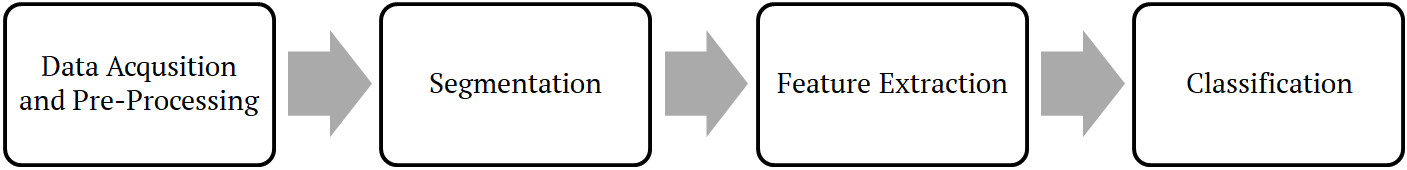
\includegraphics[width=\textwidth]{Images/erc.png} 
\vspace{-0.3cm} 
\caption[Emotion Recognition Chain]{Emotion Recognition Chain: Zeitreihen-Datens{\"a}tze werden von tragbaren Sensoren aufgenommen (Datenerfassung) und vorverarbeitet (Vorverarbeitung). Die Daten werden dann in Segmente unterteilt (Segmentierung), aus denen Merkmale extrahiert werden (Merkmalsextraktion). Mit den gewonnenen Merkmalen wird schlie{\ss}lich ein Klassifikator trainiert und anschlie{\ss}end dessen Ergebnisse bewertet (Klassifikation).}
\label{fig:erc} 
\end{figure}
%\vspace{0.5cm}


% Unterkapitel
\subsection{Datenerfassung} \label{datenerfassung-1}


In Kapitel \ref{messreihe-1-sec} wurde das verwendete Datenset bereits detailiert beschrieben, sodass hier darauf verzichtet wird. \\

% Unterkapitel 
\subsection{Vorverarbeitung} \label{vorverarbeitung-1}

Wie bereits in Kapitel \ref{vorverarbeitung-0} beschrieben, ist das Ziel der Vorverarbeitung die ”Verbesserung” der Daten f{\"u}r die nachfolgenden Schritte der ERC.
Im Rahmen des ELISE Projektes wurden Normalisierungstechniken auf dem gesamten Datensatz angewendet. 
Wir haben insbesondere die Standardnormalisierung verwendet, welche den Mittelwert der Daten auf Null setzt und die Einheitsvarianz ergibt \cite{grus15}. 
Die Formel f{\"u}r die Standardnormierung lautet:
\begin{equation} 
\Large{ {x'={\frac {x-{\overline {x}}}{\sigma }}} } 
\label{equ:norm} \end{equation} %\vspace{0.5cm}

wobei $ x $ ein Datenpunkt eines Sensorkanales, $ \overline{x} $ ist der Durchschnitt der Gesamtheit f{\"u}r diesen Sensorkanal und $ \sigma $ ist die entsprechende Standardabweichung. \\

% Unterkapitel 
\subsubsection{Segmentation} \label{segmentation-0}

Ziel dieses Schrittes ist es, Teile von Daten zu identifizieren, welche wichtige Informationen über die zu erkennenden Emotionen enthalten. 
Dies geschieht durch Filtern der Daten und Ausschließen von Segmenten, die für das Klassifizierungsproblem nicht relevant sind.
Zusätzlich wird die zu verarbeitende Datenmenge reduziert, indem Segmente eines Zeitfensters fester Größe aus den Daten extrahiert werden.
Diese Vorgeheisweise ist heute in der Praxis besonders wichtig, da sonst hardwarebedingte Einschränkungen die zu verarbeitende Datenmenge begrenzen könnten. \\

% Unterkapitel
\subsection{Merkmalsextraktion} \label{merkmalsextraftion-1}

Wie bereits in Kapitel \ref{merkmalsextraktion-subsubsec} beschrieben, ist das Ziel der Merkmalsextraktion Charakteristiken und Merkmale in den Daten zu finden, die für das
Klassifizierungsproblem von möglichst hoher Relevanz sind. Im Rahmen des ELISE Projektes haben wir verschiedene Vorgehensweisen angewendet. Im den folgenden Unterkapiteln werden diese vorgestellt. \\



% Unterkapitel 
\subsubsection{Handgefertigte Merkmale} \label{hc-features-1}
Der handgefertigten Merkmal Ansatz (enlg. "hand-crafted features approach") besteht in der Berechnung relativ einfacher Merkmale von denen vermudetet wird, dass sie für das Klassifizierungsproblem der Eingangssignale relevant sein können. Diese Vorgehensweise hat den Vorteil des einfachen Aufbaus als auch der relativ geringen benötigten Rechenleistung, wobei potentiell gute Klassifizierungsergebnisse erwarten werden. \\


Obwohl frühere Forschungsarbeiten schon handgefertigte Merkmale zur Emotionserkennung unter mithilfe physiologischer Signale getestet haben (vgl. \cite{martinez_ieee_2013}), wurde dieser Ansatz noch nie für die Erkennung dieser spezifischen Emotionen unter Verwendung dieser Kombination von Sensoren getestet.
Zusätzlich haben wir zuerst handgefertigte Merkmale getestet, um ein Basisergebnis zu liefern, mit der die Ergebnissen der anderen Ansätze vergleichen werden können.
Handgefertigte Merkmale sind in der Regel entweder einfache statistische Werte, Fourier-basierte oder selbstentwickelte Merkmale sein, die aufgrund von Vorkenntnissen der Daten verwendet werden. 
Diese Arbeit wurden statistische, Fourier-basierte und selbstentwickelte Merkmale getestet. \\

\textbf{Statistische Merkmale \\}
Die Tabelle \ref{tab:statistische} fasst die elf verschiedenen und in der Studie verwendeten statistischen Merkmale zusammen. Wir bezeichnen $\mathbf{x} = (x_1, x_2, ...., x_T) $ als Vektor, der die in einem Datenzeitfenster der Länge $T$ enthaltenen Sensorwerte für einen Sensorkanal darstellt. 


\begin{table}[h]
\begin{tabular}{| l | p{12.5cm} |}
\hline
    \textbf{Merkmalname}     &  \textbf{Definition}  \\ \hline
    
    Durchschnitt         & \vspace{0.01cm}
    $ mean(\mathbf{x}) =$ \Large{$\frac{1}{T} \sum_{k=1}^T (x_k) $} \\[0.5cm] \hline 
    
    Standard-Abweichung        & \vspace{0.01cm}
    $ \sigma(\mathbf{x}) =$ \Large{$ \sqrt{ \frac{1}{T} \sum_{k=1}^{T}{(x_k - \mu)^{2}} } $ } \\[0.5cm] \hline
    
    Maximum                   & \vspace{0.01cm}
    $ max(\mathbf{x}) = \max(x_{1},x_{2},\dots ,x_{T}) $
    \\[0.5cm] \hline
    
    Minimum                   & \vspace{0.01cm}
    $ min(\mathbf{x}) = \min(x_{1},x_{2},\dots ,x_{T}) $
    \\[0.5cm] \hline
    
    Amplitude                 & \vspace{0.01cm}
    $ A(\mathbf{x}) = max(\mathbf{x}) - min(\mathbf{x}) $ 
    \\[0.5cm] \hline
    
    25/50/75\% Perzentil      & Wert einer Menge, unter dem 25/50/75\% der Werte aus der Menge fallen. \\ \hline
    
    Interquartiler Bereich    & Differenz zwischen dem 75. und 25. Perzentil.
    \\ \hline
     
    Schräge                   & \vspace{0.01cm}
    $ \gamma _{1}(\mathbf{x}) = \operatorname{E}$ \Large{$\left[\left({\frac {X-\mu }{\sigma }}\right)^{3}\right]$ \normalsize{$=$} ${\frac {\mu _{3}}{\sigma ^{3}}}$ \normalsize{$=$} ${\frac {\operatorname {E} \left[(X-\mu )^{3}\right]}{ (\operatorname {E} \left[(X-\mu )^{2}\right])^{3/2}}}$ \normalsize{$=$} ${\frac {\kappa _{3}}{\kappa _{2}^{3/2}}} $} \vspace{0.2cm}
    \\[0.3cm] \hline
     
    Kurtosis                  & \vspace{0.01cm}
    $ \operatorname {Kurt}[\mathbf{x}] = \operatorname{E} $ \Large{$\left[\left({\frac {X-\mu }{\sigma }}\right)^{4}\right]$ \normalsize{$=$} ${\frac {\mu _{4}}{\sigma ^{4}}}$ \normalsize{$=$} ${\frac {\operatorname {E} [(X-\mu )^{4}]}{(\operatorname {E} [(X-\mu )^{2}])^{2}}} $} \vspace{0.2cm}
    \\[0.3cm] \hline
\end{tabular} 
\caption{Statistische Merkmale, die im Rahmen des ELISE-Projektes verwendet wurden. } \label{tab:statistische}
\end{table} 


\textbf{Fourier-basierte Merkmale \\}
\todo[inline]{Artur: \\
- Muss ich noch schreiben $\rightarrow$ Warten auf Julian's Antwort. \\}


\textbf{Selbstentwickelte Merkmale \\}
Es wurden zwei eigene Merkmale definiert: Nulldurchgang (engl. "zero crossing") und Anzahl der Spitzen (engl. "number of peaks"). Im Folgendem werden diese beiden Merkmale detailiert beschrieben. \\

Das Nulldurchgang-Merkmal zählt die Häufigkeit, mit der das Signal eines Sensorkanals in einem Zeitfenster die Nulllinie überschreitet.
Alle Sensorsignale wurden durch Normierung verarbeitet (vgl. Kapitel xxx) und damit wurden alle Mittelwerte auf Null zentriert.
Um zu vermeiden, dass Rauschen entlang der Nulllinie in dem Merkmal gezählt wird, wird nur ein Nulldurchgang in einer bestimmten Zeitspanne gezählt. \\


Das Spitzenzähler-Merkmal bestimmt die Anzahl von loklanen Hochpunkten im Zeitsignal.
Alle lokalen Maximen sind durch einen Onset (Startpunkt), eine Spitze und einen Offset (Endpunkt) gekennzeichnet (vgl. Abbildung \ref{fig:peaks}). 
Jedes Vorkommen einer Onset/Offset-Paarung wird hierbei als Spitze gezählt.
Onsets, Spitzen und Offsets werden durch die folgenden Operationen identifiziert \cite{BSc_Gouverneu}:

\begin{itemize} %[noitemsep]
  \item Ein Onset wird bestimmt, wenn der Wert des Signals an diesem Punkt nicht negativ ist und die Differenz zwischen ihm und dem nächsten größer als ein vordefinierter Schwellenwert (engl. "threshold") ist.

  \item Ein Offset wird bestimmt, wenn der Wert des Signals kleiner als der Wert des zuletzt gesetzten Onsets ist.

  \item Das lokale Maximum zwischen einem Onset und Offset wird als Spitze bezeichnet.
\end{itemize} \vspace{0.2cm}


\begin{figure}[h] \centering{
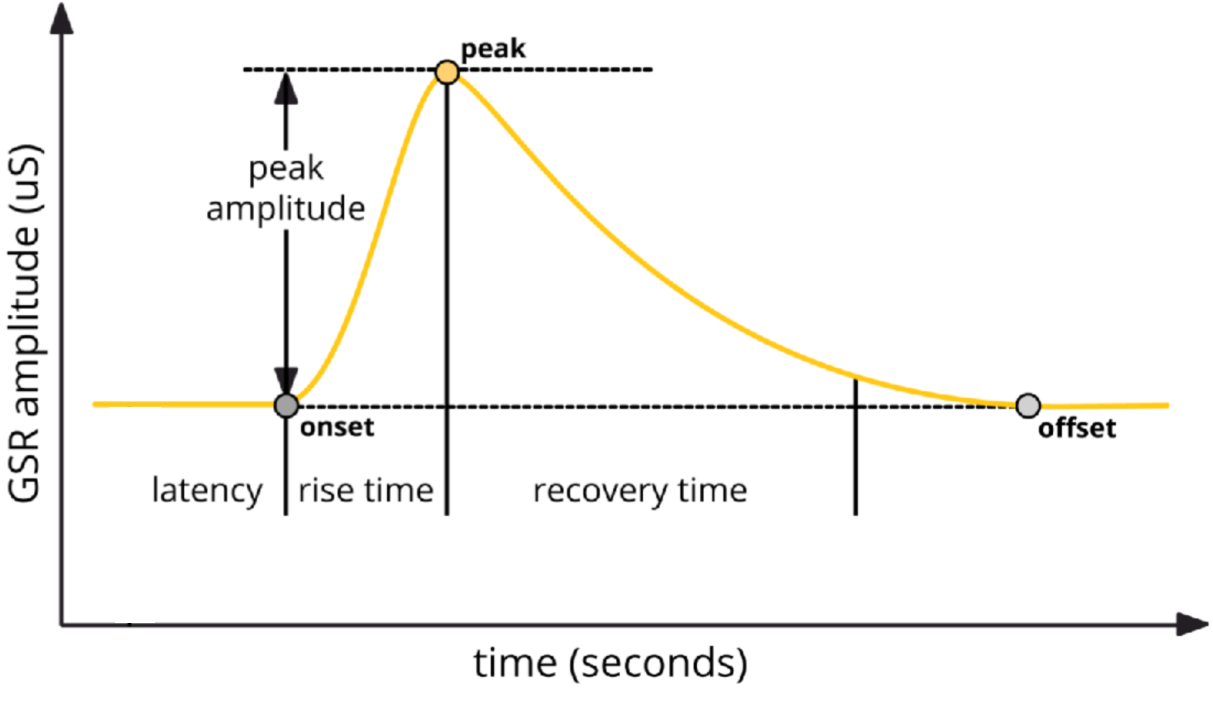
\includegraphics[width=11cm]{Images/peaks.png}}
\caption{ Spitzenzähler: Onset (Startpunkt), Spitze und Offset (Endpunkt). Jedes Paar von Onset/Offset erhöht die Anzahl der Spitzen um eins.} 
\label{fig:peaks} \end{figure} \vspace{0.5cm}


Jedes handgefertigte Merkmal wird auf einem Zeitfenster von Daten für jeden Sensorkanal unabhängig voneinander angewendet. 
Jedes Zeitfenster ist daher 117 Merkmalen zugeordnet (9 Sensorkanäle multipliziert mit 13 Merkmalen). \\





% Unterkapitel 
\subsubsection{Codebook Approach} \label{ca-1}


Die bisherige Methodik mit handgefertigten Merkmalen ist klassisch für den überwachten Lernansatz. 
Es existieren aber auch einige Nachteile. 
Das Hauptproblem besteht darin, dass nicht sichergestellt werden kann, dass die gewählten Merkmale die besten Klassifizierungsergebnisse erzielen. Damit besteht immer die Gefahr, dass möglicherweise andere Merkmalen bessere Ergebnisse liefern würden, diese handgefertigten Merkmale aber die  nicht gefunden wurden. Dieses Risiko besteht insbesondere bei der physiologischen Signalverarbeitung zur Emotionserkennung, wo die Struktur der Daten noch recht unbekannt und allgemein komplex ist. 
Eine weitere Schwierigkeit besteht darin, relevante selbstentwickelte Features ohne Expertenwissen über die Daten zu finden.
Darüber hinaus wurden noch keine gut funktionierenden State-of-the-Art handgefertigten Merkmale identifiziert.
Aus diesen Gründen ist es interessant halbautomatische und unüberwachter Ansätze der Merkmalsextraktion zu verwenden und zu testen. \\


K. Shirahama et al. \cite{kimiaki_codebook_approach_2016} schlugen eine unüberwachte Merkmalsextraktionsmethode namens Codebook Approach (CA) vor, um Merkmale aus 1D-Zeitreihensignalen zu erzeugen.
Der CA hat den Vorteil, dass formbasierte Merkmale gefunden werden können, die für das Problem der Emotionserkennung relevant sind, aber weder offensichtlich noch leicht als Mensch zu interpretieren sind. 
Der CA besteht aus drei Schritten, die in den folgenden Abschnitten erläutert werden: Codebuchkonstruktion (engl. "codebook construction"), Codewortzuordnung (engl. "codeword assignment") und der anschließenden Klassifizierung. \\


\textbf{Codebuchkonstruktion \\}
Ziel dieses Schrittes ist es, Teilsequenzen (sogenannte "Codewörter") zu bestimmen, die für die 1D-Eingangssensorik charakteristisch sind. 
Dies wird erreicht, indem Zeitfenster aus dem ursprünglichen Datensatz für jeden Sensorkanal unabhängig voneinander nach dem im Kapitel \ref{segmenation-1} definierten Segmentierungsansatz extrahiert werden.
Aus jedem so erhaltenen Zeitfenster der Größe $T$ werden kleinere Segmente der Größe $\alpha$ unterteilt.
Ein Clustering-Algorithmus wird dann auf die Menge der Segmente $\alpha$ angewendet, um Clusterzentren zu finden.
Nach der Konvergenz werden die Clusterzentren als Codewörter betrachtet und zum Aufbau einer Sammlung von Codewörtern mit dem Namen ``Codebuch'' verwendet, wie in Abbildung \ref{fig:ca_construction} aus \cite{kimiaki_codebook_approach_2016} dargestellt. 
Die Anzahl der Codewörter (d.h. die Größe des Codebuchs oder die Anzahl der Cluster) ist ein Hyperparameter des Verfahrens. Im Rahmen dieser Arbeit wurde ein k-means Clustering-Algorithmus verwendet, um die Codewörter auf den ELISE-Daten zu erhalten. \\



% Unterkapitel
\subsection{Klassifikation} \label{klassifikation-1}

Wie bereits in Kapitel \ref{grundlagen-klassifikation-0} beschrieben ist das Ziel der Klassifizierung ein Klassifizierungsmodell zu trainieren, das in der Lage ist, Objekte in den Daten in die entsprechende Klasse zuzuordnen. Die Klassen entsprechen hierbei den Emotionen, die erkannt werden sollen: Glück, Langeweile, Frustation und andere (d.h. alle Emotionen, die nicht Glück, Langeweile oder Furstation entsprechen). \\

Als erstes wird der Datensatz in ein Trainigs- und Testset  aufgeteilt. 
Es gibt keine festgelegten Regeln über die Proportionen der Sets. 
Im Allgemeinen wird das Trainingsset aber größer als das Testset gewählt.
Da die Leistungen des Klassifikators jedoch stark von der gewählten Aufteilung abhängen, ist es wichtig, sicherzustellen, dass dieser Schritt richtig durchgeführt wird.
Bei einem Datensatz mit mehreren Probanden empfiehlt sich für die Aufteilung zwischen Trainings- und Testsets die Durchführung einer Leave-One-Subjekt-Out-Cross-Validierung (LOSOCV).
Die Idee besteht darin, $N$ verschiedene Aufteilungen des Datensatzes vorzunehmen, wobei $N$ die Anzahl der Personen ist, die Daten für den Datensatz bereitgestellt haben. 
Für jeden dieser Splits wird der Testset aus den Daten eines Probanden aufgebaut, während die Daten der anderen Probanden das Trainingsset bilden. 
Anschließend wird ein Klassifizierer erstellt und ausgewertet. Dies wird für alle Probanden wiederholt, d.h. $N$ mal.
Die so erhaltenen $N$-Bewertungskennzahlen (eine pro Proband) können dann gemittelt werden, um eine Gesamtbewertung des Modells zu erhalten.
Es ist wichtig zu beachten, dass der LOSOCV-Ansatz bei einer hohen Anzahl von Probanden sehr rechenintensiv sein kann. \\

\begin{figure}[h] \centering{
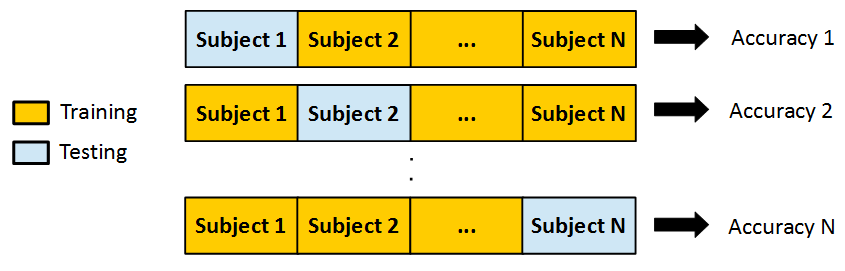
\includegraphics[width=15cm]{Images/LOSOCV.png} 
\caption{ Leave-One-Subjekt-Out-Cross-Validation (LOSOCV): $N$ entspricht der Anzahl der Probanden. Für jeden Split wird ein Testset aus den Daten eines Probanden aufgebaut, während die Daten der anderen Probanden einen Trainingsset bilden. Dieser Vorgang wird für die Daten jedes Probanden durchgeführt. }}
\label{fig:losocv} \end{figure} \vspace{0.5cm}



